%********************************************************************************************************
%  Tipo de documento
%********************************************************************************************************
\documentclass[a4paper,11pt]{article}
%********************************************************************************************************
%  Paquetes empleados
%********************************************************************************************************
\usepackage[utf8]{inputenc} % Esto es para poder escribir acentos directamente
\usepackage[spanish]{babel} % Esto es para que el LaTeX sepa que el texto está en español
\usepackage{amsmath, amsthm, amsfonts} % Paquetes de la AMS
\usepackage{fancyhdr}
\usepackage{enumerate} % Paquete de enumeraciones
\usepackage{hyperref}
\usepackage{graphicx}
\usepackage{colortbl}
\usepackage{pdflscape}

% Renombrando
\renewcommand\tablename{Tabla}
\renewcommand\figurename{Figura}
\renewcommand\contentsname{Tabla de contenidos}
\renewcommand\refname{Bibliografía}

\pagestyle{fancy}
\fancyhf{}
% En lo siguiente, fancyhead sirve para configurar la cabecera, fancyfoot para el pie.
% Justificación: C=centered, R=right, L=left, (nada)=LRC
% Página: O=odd, E=even, (nada)=OE
\fancyhead[C]{\rightmark}
\fancyhead[C]{\leftmark}
\fancyfoot[C]{\thepage}

% Modifica el ancho de las lí­neas de cabecera y pie
\renewcommand{\headrulewidth}{0.4pt}
\renewcommand{\footrulewidth}{0.4pt}
\setlength{\headheight}{1.5\headheight} % Aumenta la altura del encabezado en una vez y media


%********************************************************************************************************
\begin{document}
    %***************************************************************************************************
	%  Portada
	%***************************************************************************************************
	\begin{titlepage}
		\begin{center}
			
\includegraphics[width=375px]{Universidad.png} \\
            
\includegraphics[width=250px]{logo_cordosoft.png} \\
            
\includegraphics[width=200px]{conservart_logo.png} \\
			\textbf{\LARGE Documento de especificación} \\
			\\
			\textbf{}
			\\
			\textbf{\Large SDJS - RCPTTE} \\
			\\
			\textbf{}
			\\
			\textbf{Autores}
			\\
			\textbf{}
			\\
			\begin{tabular}{l l}
				\textbf{Raul Arroyo Lubián} & \textbf{i02arlur@uco.es} \\	
				\textbf{Pedro Daniel López González} & \textbf{i02logop@uco.es} \\
				\textbf{Alfonso Lacalle García} & \textbf{i52lagaa@uco.es} \\
			\end{tabular}
			\\
			\textbf{}
			\\
			\textbf{}
			\\
			\begin{tabular}{l l}
				\textbf{Fecha de creación:} & \textbf{17 de mayo de 2013} \\
				\textbf{Fecha de última modificación:} & \textbf{\today } \\
			\end{tabular}
		\end{center}
    \end{titlepage}
	\newpage
	%***************************************************************************************************
	%  Indice
	%***************************************************************************************************
	\tableofcontents
	\pagenumbering{arabic}
	\newpage
	%***************************************************************************************************
	% Contenido
	%***************************************************************************************************
	\section{Introducción}
	Cordosoft es una empresa cordobesa dedicada al desarrollo de Sistemas Basados
	en Conocimiento (SBC) y Desarrollo Web a medida. Su principal forma de negocio
	es la primera ya que es la única empresa nacional dedicada a este ámbito. La
	fecha de creación de la empresa Cordosoft data del 1 de Abril del 2013.\\
	
	Entre los objetivos de la empresa, se encuentran algunos como dar un servicio y
	desarrollo de calidad al cliente, garantizando el mejor rendimiento de sus
	sistemas en el dominio especificado y ser un referente tanto nacional como
	internacional en el sector de los desarrollos e investigación de los Sistemas
	Basados en conocimiento.\\
	
	Como no podía ser de otro modo ya que la empresa se dedica tanto a desarrollo
	de Sistemas Basados en Conocimiento como Desarrollos WEB, todos los proyectos
	que se realizan tiene una base fundamentada en tecnologías WEB, como son HTML5,
	CSS3 y Javascript.\\
	
	El proyecto que es el presente documento vamos a detallar viene a petición de
	una empresa dedicada a la conservación y restauración de obras de arte y
	patrimonio urbano. Se trata de ConservART, una empresa creada el 5 de Mayo del
	2001 conocida nacionalmente por su calidad en la restauración de cualquier tipo
	de obra de arte. Entre sus restauraciones más famosas, podemos encontrar el
	Cristo de Borja, comunmente conocido como 'Ecce Hommo' la cual dió la vuelta al
	mundo por su exactitud y perfección en las técnicas empleadas y recuperando una
	obra dañada por el paso de los siglos, haciendola parecer la original.\\
	
	ConservART acudió a Cordosoft con la idea de propagar sus fronteras más allá de
	lo nacional, la cual actualmente era una tarea ardúa puesto que tardaban
	demasiado en encontrar todos los posibles problemas que afectaban a una obra de
	arte para su posterior restauración. Su idea era un sistema capaz de
	diagnosticar los problemas que presenta una determinada obra de arte a partir
	de unos fallos u observaciones realizadas por un restaurador. Esto haría que
	los aprendices del área de formación no dependieran continuamente de un experto
	en la materia para ayudarles con su labor y agilizar así el proceso de
	restauración, pudiendo aceptar más encargos de restauraciones. \\
	
	Como resultado a la petición, Cordosoft se puso manos a la obra y empezó a
	desarrollar el sistema que se detalla en el presente documento, utilizando la
	metodología de CommonKADS para la obtención del conocimiento.
	
	\newpage
	\section{Modelado de contexto}
		\subsection{Modelo de organización}
			\subsubsection{Formulario OM-1}
			\begin{center}
				\begin{tabular}{| p{2.9cm} | p{8.5cm} |}
					\hline
					\cellcolor[RGB]{224,233,250}\textbf{Problemas y oportunidades} &
					Muchas veces era complicado ponerse en contacto con los expertos. El equipo
					de restauración tenían mucho trabajo atrasado y se acumulaban tareas que hacer.\\
					\cellcolor[RGB]{224,233,250}& La empresa de arte no podía aceptar nuevos
					pedidos.\\
					\cellcolor[RGB]{224,233,250}& Las posibilidades de expansión de esta
					empresa eran muy complicadas, incluso teniendo personal más que cualificado.\\
					\cellcolor[RGB]{224,233,250}& La empresa de arte tiene ya clientes que
					están deseando trabajar con ellas, el trabajo acumulado le impide a esta empresa acceder a estos nuevos
					contratos.\\
					\cellcolor[RGB]{224,233,250}& Discusiones personales en los expertos que
					hacen que muchas veces sea imposible empezar un trabajo de restauración.\\
					\cellcolor[RGB]{224,233,250}& La formación de nuevos técnicos es costosa se
					desea conservar el conocimiento en la detección de fallos de las obras de arte.\\
					\hline
					\cellcolor[RGB]{224,233,250}\textbf{Contexto organizacional} &
					Empresa dedicada al estudio, conservación y restauración de obras de arte.\\
					\hline
					\cellcolor[RGB]{224,233,250}\textbf{Soluciones} & \textbf{Solución 1:}
					seguir funcionando como hasta ahora.\\
					\cellcolor[RGB]{224,233,250}& \textbf{Solución 2:} formar en el diagnóstico
					a los restauradores de la empresa.\\
					\cellcolor[RGB]{224,233,250}& \textbf{Solución 3:} desarrollo de un SBC
					para guiar la entrevista inicial con el cliente de manera que se obtenga la mayor y mejor información posible sobre el fallo del obra de arte. Este SBC podría ser utilizado bien por el cliente vía Web o bien por el/los restaurador/es, en función del medio que estos empleen para solicitar la restauración.\\
					\cellcolor[RGB]{224,233,250}& \textbf{Solución 4:} desarrollo de un SBC que
					servirá como guía al servicio de asistencia técnica en los procesos de restauración y que será usado por los restauradores.\\
					\hline
				\end{tabular}
			\end{center}
			\newpage
			\subsubsection{Formulario OM-2}
			\begin{center}
				\begin{tabular}{| p{2.5cm} | p{9cm} |}
					\hline
					\cellcolor[RGB]{224,233,250}\textbf{Estructura} & El organigrama
					corporativo en el que se detallan los departamentos de interes.\\
					\cellcolor[RGB]{224,233,250}& El \textbf{Área de Administración} se encarga
					de las tareas administrativas de la empresa.\\
					\cellcolor[RGB]{224,233,250}& El \textbf{Área de Formación} en la que se
					forma a los distintos empleados de la empresa mediante cursos y talleres.\\
					\cellcolor[RGB]{224,233,250}& El \textbf{Área de Conservación y
					Restauración} que es la encargada en restaurar y conservar distintas piezas de arte.\\
					\cellcolor[RGB]{224,233,250}& El \textbf{Área de Investigación} se dedica a
					la investigación de nuevos procesos para la conservación y estudio de obras de arte.\\
					\cellcolor[RGB]{224,233,250}& El \textbf{Área de Bellas Artes} se dedica al
					estudio histórico de las distintas obras de arte gestionadas por la empresa.\\
					\hline
					\cellcolor[RGB]{224,233,250}\textbf{Procesos} & Proceso de asistencia
					técnica, atención al cliente, restauración de obras de arte, análisis en laboratorio de fragmentos de obras de arte, formación de empleados.\\
					\hline
					\cellcolor[RGB]{224,233,250}\textbf{Personal} & Administrativos,
					coordinador restaurador, restaurador (pintura y soporte), coordinador jurídico, coordinador económico, coordinador de bellas artes, historiador, biólogo y químico.\\
					\hline
					\cellcolor[RGB]{224,233,250}\textbf{Recursos} & Los recursos de la empresa
					son prácticamente ilimitados para el trabajo de restauración y conservación de arte. Si no disponen de algo, no escatimarán en gastos para obtenerlo.\\
					\hline
					\cellcolor[RGB]{224,233,250}\textbf{Conocimiento} & La empresa dispone de
					una gran cantidad de conocimiento a través de sus expertos sobre la conservación y restauración de piezas de arte.\\
					\hline
					\cellcolor[RGB]{224,233,250}\textbf{Cultura y potencial} & La empresa
					trabaja a nivel nacional debido a sus limitaciones actuales. Con la implementación del nuevo Sistema Basado en Conocimiento podrá llegar a trabajar a nivel internacional, pudiendo recibir pedidos de cualquier cliente, tanto público como privado del propio sector.\\
					\hline
				\end{tabular}\\
				\newpage
				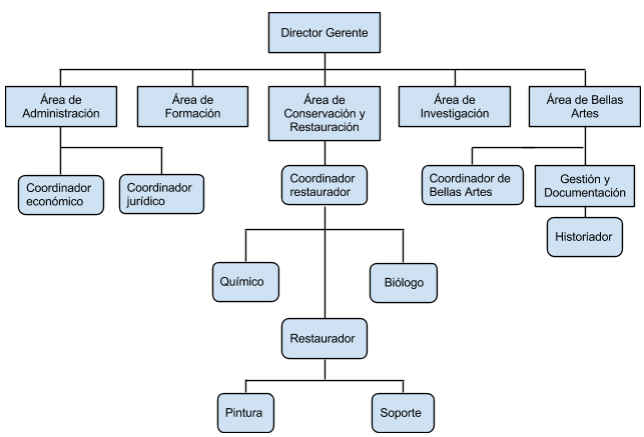
\includegraphics[width=350px]{organigrama.png} \\
			\end{center}
			\newpage
			\begin{landscape}
			\subsubsection{Formulario OM-3}
			\begin{center}
				\begin{tabular}{| l | p{4cm} | p{2.8cm} | p{2cm} | p{2cm} | p{3cm} |
				p{2.2cm} |}
					\hline
					\cellcolor[RGB]{224,233,250}\textbf{Nº} &
					\cellcolor[RGB]{224,233,250}\textbf{Tarea} &
					\cellcolor[RGB]{224,233,250}\textbf{Realizada por} &
					\cellcolor[RGB]{224,233,250}\textbf{¿Donde?} &
					\cellcolor[RGB]{224,233,250}\textbf{Recursos de conocimiento} &
					\cellcolor[RGB]{224,233,250}\textbf{¿Intensivo en conocimiento?} &
					\cellcolor[RGB]{224,233,250}\textbf{Importancia}\\
					\hline
					1 & Negociación de la obra de arte (valoración) & Director gerente &
					Despacho del director & Si & Si & Si\\
					\hline
					2 & Gestión de clientes & Área de administración & Área de administración
					& Si & No & Si\\
					\hline
					3 & Manipulación de personal & Área de administración & Área de
					administración & No & No & Si\\
					\hline
					4 & Información histórica de la obra de arte & Área de bellas artes & Área
					de bellas artes & Si & No & Si\\
					\hline
				\end{tabular}
			\end{center}
			\end{landscape}
			\newpage
			\begin{landscape}
			\begin{center}
				\begin{tabular}{| l | p{4cm} | p{2.8cm} | p{2cm} | p{2cm} | p{3cm} |
				p{2.2cm} |}
					\hline
					\cellcolor[RGB]{224,233,250}\textbf{Nº} &
					\cellcolor[RGB]{224,233,250}\textbf{Tarea} &
					\cellcolor[RGB]{224,233,250}\textbf{Realizada por} &
					\cellcolor[RGB]{224,233,250}\textbf{¿Donde?} &
					\cellcolor[RGB]{224,233,250}\textbf{Recursos de conocimiento} &
					\cellcolor[RGB]{224,233,250}\textbf{¿Intensivo en conocimiento?} &
					\cellcolor[RGB]{224,233,250}\textbf{Importancia}\\
					\hline
					5 & Prediagnóstico de la obra de arte & Área de conservación &
					Deslocalizado & Si & Si & Si\\
					\hline
					6 & Diagnóstico de la obra de arte & Área de conservación y restauración &
					Taller & Si & Si & Si\\
					\hline
					7 & Reparacion de la obra de arte & Área de conservación y restauración &
					Taller & Si & Si & Si\\
					\hline
					8 & Elaboración de presupuesto & Área de administración & Área de
					administración & No & No & No\\
					\hline
				\end{tabular}
			\end{center}
			\end{landscape}
			\newpage
			\begin{landscape}
			\subsubsection{Formulario OM-4}
			\begin{center}
				\begin{tabular}{| p{5cm} | p{2.4cm} | p{2cm} | p{2cm} | p{2cm} | p{2cm} |
				p{2cm} |}
					\hline
					\cellcolor[RGB]{224,233,250}\textbf{Recurso de conocimiento} &
					\cellcolor[RGB]{224,233,250}\textbf{Pertenece a} &
					\cellcolor[RGB]{224,233,250}\textbf{Usado en} &
					\cellcolor[RGB]{224,233,250}\textbf{¿Forma correcta?} &
					\cellcolor[RGB]{224,233,250}\textbf{¿Lugar correcto?} &
					\cellcolor[RGB]{224,233,250}\textbf{¿Tiempo correcto?} &
					\cellcolor[RGB]{224,233,250}\textbf{¿Calidad concreta?}\\
					\hline
					Negociación de la obra de arte & Director gerente & 5,6,7,8 & Si & Si & No, a
					veces se tarda demasiado. & Si.\\
					\hline
					Prediagnóstico de la obra de arte & Area de conservacion & 6,7,8 & Si & No,
					a veces se hace fuera del taller. & No, a veces se tarda demasiado. & Si\\
					\hline
					Diagnóstico de la obra de arte & Área de conservación & 7,8 & Si & Si & No,
					se tarda demasiado. & Si\\
					\hline
					Restauración de la obra de arte & Área de conservación & & Si & Si & Si & Si\\
					\hline
				\end{tabular}
			\end{center}
			\end{landscape}
			\newpage
			\subsubsection{Formulario OM-5}
			\begin{center}
				\begin{tabular}{| p{4.5cm} | p{7cm} |}
					\hline
					\cellcolor[RGB]{224,233,250}\textbf{Viabilidad empresarial} & 
					\textbf{1. ¿Cuáles son los beneficios para la organización con la adopción
					de la solución?}\\
					\cellcolor[RGB]{224,233,250}& La empresa podrá acceder a nuevos proyectos
					ya que el SBC agilizará el proceso de diagnóstico.\\
					\cellcolor[RGB]{224,233,250}& \\
					\cellcolor[RGB]{224,233,250}& \textbf{2. ¿Cómo es el valor añadido
					esperado?}\\
					\cellcolor[RGB]{224,233,250}& Se espera que gracias al SBC se podrá
					realizar todos los proyectos que hasta ahora no han podido ser aceptados. Gracias a esto ConservArt podrá acceder a proyectos internacionales.\\
					\cellcolor[RGB]{224,233,250}& \\
					\cellcolor[RGB]{224,233,250}& \textbf{3. ¿Se requieren cambios
					organizacionales?}\\
					\cellcolor[RGB]{224,233,250}& No\\
					\hline
					\cellcolor[RGB]{224,233,250}\textbf{Viabilidad técnica} & 
					\textbf{1. ¿Existen aspectos críticos relativos al tiempo, calidad,
					recursos necesarios, etc?}\\
					\cellcolor[RGB]{224,233,250}& Si, el tiempo que se dedicaba para el
					diagnóstico era demasiado alto.
					Gracias al SBC estos tiempos disminuyen mucho.\\
					\cellcolor[RGB]{224,233,250}& \\
					\cellcolor[RGB]{224,233,250}& \textbf{2. ¿Cómo es de compleja la
					interacción con el usuario?}\\
					\cellcolor[RGB]{224,233,250}& La interacción con el usuario no es nada
					compleja. La aplicación es bastante intuitiva.\\
					\cellcolor[RGB]{224,233,250}& \\
					\cellcolor[RGB]{224,233,250}& \textbf{3. ¿Qué complejidad tiene la solución
					propuesta desde el punto de vista del conocimiento y los procesos de razonamiento desarrollado?}\\
					\cellcolor[RGB]{224,233,250}& La solución propuesta presenta la tarea de
					diagnóstico.
					Ésta viene detallada en la librería de CommonKads.\\
					\hline
				\end{tabular}
			\end{center}
			\newpage
			\begin{center}
				\begin{tabular}{| p{4.5cm} | p{7cm} |}
					\hline
					\cellcolor[RGB]{224,233,250}\textbf{Viabilidad del proyecto} & 
					\textbf{1. ¿Existe el compromiso por parte de ConservArt para llevar a
					cabo el proyecto?}\\
					\cellcolor[RGB]{224,233,250}& Si, la empresa se implica por completo.\\
					\cellcolor[RGB]{224,233,250}& \\
					\cellcolor[RGB]{224,233,250}& \textbf{2. ¿Está disponible el conocimiento y
					las capacidades requeridas?}\\
					\cellcolor[RGB]{224,233,250}& Si, están disponibles.\\
					\cellcolor[RGB]{224,233,250}& \\
					\cellcolor[RGB]{224,233,250}& \textbf{3. ¿Son realistas las expectativas
					relacionadas con el proyecto y los resultados?}\\
					\cellcolor[RGB]{224,233,250}& Si, ConservArt es una empresa en expansión y
					muchos clientes están esperando sus servicios.\\
					\hline
					\cellcolor[RGB]{224,233,250}\textbf{Acciones propuestas} & 
					\textbf{1. ¿Cuáles son los resultados, costes y beneficios esperados?}\\
					\cellcolor[RGB]{224,233,250}& El coste del sistema basado en conocimiento
					es alto en sus inicios. A la larga, sin embargo, permitirá a la empresa abordar proyectos en todo el
					mundo.\\
					\cellcolor[RGB]{224,233,250}& \\
					\cellcolor[RGB]{224,233,250}& \textbf{2. ¿Qué acciones se deben tomar
					dentro del proyecto para alcanzar dicha solución?}\\
					\cellcolor[RGB]{224,233,250}& ConservArt debe implicarse por completo con
					la realización del Sistema Basado en Conocimiento si quiere que el desarrollo de este tenga el éxito deseado.\\
					\cellcolor[RGB]{224,233,250}& \\
					\cellcolor[RGB]{224,233,250}& \textbf{3. Si las circunstancias que rodean a
					la organización cambian (tanto externas como internas), ¿bajo qué condiciones es apropiado
					reconsiderar las decisiones tomadas?}\\
					\cellcolor[RGB]{224,233,250}& La creación del Sistema Basado en
					Conocimiento afecta sólo a tareas agrupadas en dos departamentos. estos departamentos son pilares de la organización así que siempre deben formar parte de ella. Eso hace que la aplicación no se vea afectada por ninguna de estas causas.\\
					\hline
				\end{tabular}
			\end{center}
		\newpage
		\subsection{Modelo de tareas}
			\subsubsection{Formulario TM-1}
			\begin{center}
				\begin{tabular}{| l | p{6.5cm} |}
					\hline
					\cellcolor[RGB]{224,233,250}\textbf{Tarea} & Negociación de la obra de
					arte.\\
					\hline
					\cellcolor[RGB]{224,233,250}\textbf{Organización} & Forma parte del proceso
					de restauración de obras de arte. Si la negociación es satisfactoria la empresa de restauración empezará a trabajar con la obra.\\
					\hline
					\cellcolor[RGB]{224,233,250}\textbf{Objetivo y valor} & El objetivo es
					valorar si una propuesta de negocio es interesante y viable para la empresa.\\
					\hline
					\cellcolor[RGB]{224,233,250}\textbf{Dependencias y flujos} & \textbf{Tareas
					precedentes:} ninguna.\\
					\cellcolor[RGB]{224,233,250}& \textbf{Tareas siguientes:} Prediagnóstico,
					Diagnóstico, Elaborar presupuesto y Restauración de la obra.\\
					\hline
					\cellcolor[RGB]{224,233,250}\textbf{Objetos manipulados} & \textbf{Objetos
					de entrada:} información sobre el cliente y sobre la obra de arte que va a ser valorada.\\
					\cellcolor[RGB]{224,233,250}& \textbf{Objetos de salida:} aceptación o no
					de la negociación.\\
					\hline
					\cellcolor[RGB]{224,233,250}\textbf{Tiempo y control} &
					\textbf{Frecuencia:} cada vez que un cliente solicita la restauración de una obra de arte.\\
					\hline
					\cellcolor[RGB]{224,233,250}\textbf{Agentes} & \textbf{Agente humano:}
					director general, personal administrativo.\\
					\hline
					\cellcolor[RGB]{224,233,250}\textbf{Conocimiento y capacidad} & Los
					recursos de conocimiento establecidos en OM3.\\
					\hline
					\cellcolor[RGB]{224,233,250}\textbf{Recursos} & Teléfono y computadora para
					comunicación con el cliente.\\
					\hline
					\cellcolor[RGB]{224,233,250}\textbf{Calidad y eficiencia} & La tarea deberá
					seguir la normativa de calidad marcada por la empresa, documentada gracias al certificado de
					calidad. El sistema irá afinando su comportamiento conforme al estudio de
					nuevos casos de valoración.\\
					\hline
				\end{tabular}
			\end{center}
			\newpage
			\begin{center}
				\begin{tabular}{| l | p{6.5cm} |}
					\hline
					\cellcolor[RGB]{224,233,250}\textbf{Tarea} & Prediagnóstico de la obra de
					arte.\\
					\hline
					\cellcolor[RGB]{224,233,250}\textbf{Organización} & Forma parte del proceso
					de restauración de obras de arte. Es responsabilidad del departamento de Área de Conservación y
					Restauración.\\
					\hline
					\cellcolor[RGB]{224,233,250}\textbf{Objetivo y valor} & El objetivo es
					realizar una posible localización del problema en función de los datos del cliente.\\
					\hline
					\cellcolor[RGB]{224,233,250}\textbf{Dependencias y flujos} & \textbf{Tareas
					precedentes:} ninguna.\\
					\cellcolor[RGB]{224,233,250}& \textbf{Tareas siguientes:} Elaborar
					presupuesto, restauración y diagnóstico de la obra de arte.\\
					\hline
					\cellcolor[RGB]{224,233,250}\textbf{Objetos manipulados} & \textbf{Objetos
					de entrada:} datos del problema de la obra de arte mediante descripción y/o fotos.\\
					\cellcolor[RGB]{224,233,250}& \textbf{Objetos de salida:} posible causa del
					fallo, análisis insuficiente necesita un diagnóstico en taller.\\
					\hline
					\cellcolor[RGB]{224,233,250}\textbf{Tiempo y control} &
					\textbf{Frecuencia:} cada vez que se acepta una negociación.\\
					\hline
					\cellcolor[RGB]{224,233,250}\textbf{Agentes} & Personal administrativo,
					restaurador.\\
					\hline
					\cellcolor[RGB]{224,233,250}\textbf{Conocimiento y capacidad} & Los
					recursos de conocimiento establecidos en OM-3.\\
					\hline
					\cellcolor[RGB]{224,233,250}\textbf{Recursos} & Equipo informático con una
					pantalla con una gran resolución. Proyector de hologramas.\\
					\hline
					\cellcolor[RGB]{224,233,250}\textbf{Calidad y eficiencia} & La tarea deberá
					seguir la normativa de calidad marcada por la empresa, documentada gracias al certificado de calidad. El sistema irá afinando su comportamiento conforme al estudio de nuevos casos de diagnosis , valoración y restauración introducidos.\\
					\hline
				\end{tabular}
			\end{center}
			\newpage
			\begin{center}
				\begin{tabular}{| l | p{6.5cm} |}
					\hline
					\cellcolor[RGB]{224,233,250}\textbf{Tarea} & Diagnóstico de la obra de
					arte.\\
					\hline
					\cellcolor[RGB]{224,233,250}\textbf{Organización} & Forma parte del proceso
					de restauración de obras de arte. Es responsabilidad del departamento de Área de Conservación y
					Restauración.\\
					\hline
					\cellcolor[RGB]{224,233,250}\textbf{Objetivo y valor} & El objetivo es
					realizar una posible localización del problema analizando la obra de arte con detalle.\\
					\hline
					\cellcolor[RGB]{224,233,250}\textbf{Dependencias y flujos} & \textbf{Tareas
					precedentes:} Negociación de la obra de arte, prediagnóstico de la obra de arte.\\
					\cellcolor[RGB]{224,233,250}& \textbf{Tareas siguientes:} Restauración de
					la obra de arte.\\
					\hline
					\cellcolor[RGB]{224,233,250}\textbf{Objetos manipulados} & \textbf{Objetos
					de entrada:} datos del fallo de la obra de arte.\\
					\cellcolor[RGB]{224,233,250}& \textbf{Objetos de salida:} posibles causas
					del problema.\\
					\hline
					\cellcolor[RGB]{224,233,250}\textbf{Tiempo y control} &
					\textbf{Frecuencia:} Cada vez que es necesario un diagnóstico detallado.\\
					\hline
					\cellcolor[RGB]{224,233,250}\textbf{Agentes} & Restaurador.\\
					\hline
					\cellcolor[RGB]{224,233,250}\textbf{Conocimiento y capacidad} & Los
					recursos de conocimiento establecidos en OM-3.\\
					\hline
					\cellcolor[RGB]{224,233,250}\textbf{Recursos} & Taller con todos los
					elementos necesarios para la realización del diagnóstico.\\
					\hline
					\cellcolor[RGB]{224,233,250}\textbf{Calidad y eficiencia} & La tarea deberá
					seguir la normativa de calidad marcada por la empresa, documentada gracias al certificado de calidad. El sistema irá afinando su comportamiento conforme al estudio de nuevos casos de diagnosis, valoración y restauración introducidos.\\
					\hline
				\end{tabular}
			\end{center}
			\newpage
			\begin{center}
				\begin{tabular}{| l | p{6.5cm} |}
					\hline
					\cellcolor[RGB]{224,233,250}\textbf{Tarea} & Restauración de la obra de
					arte.\\
					\hline
					\cellcolor[RGB]{224,233,250}\textbf{Organización} & Es responsabilidad del
					departamento de Área de Conservación y Restauración.\\
					\hline
					\cellcolor[RGB]{224,233,250}\textbf{Objetivo y valor} & El objetivo es
					realizar una restauración de la obra de arte de la manera más eficiente, correcta y utilizando todo el conocimiento que poseen los expertos de la empresa.\\
					\hline
					\cellcolor[RGB]{224,233,250}\textbf{Dependencias y flujos} & \textbf{Tarea
					precedentes:} Negociación de la obra de arte, prediagnóstico de la obra de arte, diagnóstico de la obra de arte.\\
					\cellcolor[RGB]{224,233,250}& \textbf{Tareas siguientes:} ninguna.\\
					\hline
					\cellcolor[RGB]{224,233,250}\textbf{Objetos manipulados} & \textbf{Objetos
					de entrada:} datos de los distintos problemas.\\
					\cellcolor[RGB]{224,233,250}& \textbf{Objetos de salida:} soluciones a esos
					problemas.\\
					\hline
					\cellcolor[RGB]{224,233,250}\textbf{Tiempo y control} &
					\textbf{Frecuencia:} cada vez que se tenga una obra de arte dispuesta a restaurar.\\
					\hline
					\cellcolor[RGB]{224,233,250}\textbf{Agentes} & Restaurador.\\
					\hline
					\cellcolor[RGB]{224,233,250}\textbf{Conocimiento y capacidad} & Los
					recursos de conocimiento establecidos en OM-3.\\
					\hline
					\cellcolor[RGB]{224,233,250}\textbf{Recursos} & Taller con todos los
					elementos necesarios para la reparación de la obra de arte.\\
					\hline
					\cellcolor[RGB]{224,233,250}\textbf{Calidad y eficiencia} & La tarea deberá
					seguir la normativa de calidad marcada por la empresa, documentada gracias al certificado de calidad. El sistema irá afinando su comportamiento conforme al estudio de nuevos casos de diagnosis, valoración y restauración introducidos.\\
					\hline
				\end{tabular}
			\end{center}
			\newpage
			\subsubsection{Formulario TM-2}
			\begin{center}
				\begin{tabular}{| p{3cm} | p{8.85cm} |}
					\hline
					\cellcolor[RGB]{224,233,250}\textbf{Nombre} & Procedimiento de técnicos en
					la detección y restauración de obras de arte.\\
					\hline
					\cellcolor[RGB]{224,233,250}\textbf{Poseído por} & Restauradores del
					departamento de Área de conservación y restauración.\\
					\hline
					\cellcolor[RGB]{224,233,250}\textbf{Usado en} & 5, 6, 7\\
					\hline
					\cellcolor[RGB]{224,233,250}\textbf{Dominio} & Restauración y Conservación
					de pintura al temple al huevo sobre tabla sin entelar.\\
					\hline
				\end{tabular}
				\\
				\textbf{}
				\\
				\\
				\textbf{}
				\\
				\begin{tabular}{| p{6.3cm} | l | p{3.8cm} |}
					\hline
					\cellcolor[RGB]{224,233,250}\textbf{Naturaleza del conocimiento} &
					\cellcolor[RGB]{224,233,250}\textbf{(si/no)} &
					\cellcolor[RGB]{224,233,250}\textbf{¿Cuello de botella?}\\
					\hline
					\cellcolor[RGB]{224,233,250}\textbf{Forma, riguroso} & No & No\\
					\hline
					\cellcolor[RGB]{224,233,250}\textbf{Empírico, cuantitativo} & No & No\\
					\hline
					\cellcolor[RGB]{224,233,250}\textbf{Específico del dominio} & Si & No\\
					\hline
					\cellcolor[RGB]{224,233,250}\textbf{Basado en la experiencia} & Si & Si \\
					\hline
					\cellcolor[RGB]{224,233,250}\textbf{Basado en la acción} & Si & Si \\
					\hline
					\cellcolor[RGB]{224,233,250}\textbf{Incompleto} & Si & Si \\
					\hline
					\cellcolor[RGB]{224,233,250}\textbf{Incierto, puede ser incorrecto} & Si &
					Si \\
					\hline
					\cellcolor[RGB]{224,233,250}\textbf{Cambia con rapidez} & No & No\\
					\hline
					\cellcolor[RGB]{224,233,250}\textbf{Difícil de verificar} & Si & Si \\
					\hline
					\cellcolor[RGB]{224,233,250}\textbf{Tácito, difícil de transferir} & Si &
					Si \\
					\hline
					\cellcolor[RGB]{224,233,250}\textbf{Forma de conocimiento} &
					\cellcolor[RGB]{224,233,250}\textbf{(si/no)} &
					\cellcolor[RGB]{224,233,250}\textbf{¿Cuello de botella?}\\
					\hline
					\cellcolor[RGB]{224,233,250}\textbf{Mental} & Si & No\\
					\hline
					\cellcolor[RGB]{224,233,250}\textbf{Papel} & Si & Si\\
					\hline
					\cellcolor[RGB]{224,233,250}\textbf{Electrónica} & Si & No\\
					\hline
					\cellcolor[RGB]{224,233,250}\textbf{Habilidades} & Si & No\\
					\hline
					\cellcolor[RGB]{224,233,250}\textbf{Otros} & No & No\\
					\hline
					\cellcolor[RGB]{224,233,250}\textbf{Disponibilidad del conocimiento} &
					\cellcolor[RGB]{224,233,250}\textbf{(si/no)} &
					\cellcolor[RGB]{224,233,250}\textbf{¿Cuello de botella?}\\
					\hline
					\cellcolor[RGB]{224,233,250}\textbf{Limitaciones en tiempo} & Si & No\\
					\hline
					\cellcolor[RGB]{224,233,250}\textbf{Limitaciones en espacio} & No & No\\
					\hline
					\cellcolor[RGB]{224,233,250}\textbf{Limitaciones en acceso} & No & No\\
					\hline
					\cellcolor[RGB]{224,233,250}\textbf{Limitaciones en calidad} & No & No\\
					\hline
					\cellcolor[RGB]{224,233,250}\textbf{Limitaciones en forma} & No & No\\
					\hline
				\end{tabular}
			\end{center}
			\newpage
			\begin{center}
				\begin{tabular}{| p{3cm} | p{8.85cm} |}
					\hline
					\cellcolor[RGB]{224,233,250}\textbf{Nombre} & Procedimiento de valoración
					de un proyecto.\\
					\hline
					\cellcolor[RGB]{224,233,250}\textbf{Poseído por} & Director gerente.\\
					\hline
					\cellcolor[RGB]{224,233,250}\textbf{Usado en} & 1\\
					\hline
					\cellcolor[RGB]{224,233,250}\textbf{Dominio} & Restauración y Conservación
					de pintura al temple al huevo sobre tabla sin entelar.\\
					\hline
				\end{tabular}
				\\
				\textbf{}
				\\
				\\
				\textbf{}
				\\
				\begin{tabular}{| p{6.3cm} | l | p{3.8cm} |}
					\hline
					\cellcolor[RGB]{224,233,250}\textbf{Naturaleza del conocimiento} &
					\cellcolor[RGB]{224,233,250}\textbf{(si/no)} &
					\cellcolor[RGB]{224,233,250}\textbf{¿Cuello de botella?}\\
					\hline
					\cellcolor[RGB]{224,233,250}\textbf{Forma, riguroso} & No & No\\
					\hline
					\cellcolor[RGB]{224,233,250}\textbf{Empírico, cuantitativo} & No & No\\
					\hline
					\cellcolor[RGB]{224,233,250}\textbf{Específico del dominio} & Si & Si\\
					\hline
					\cellcolor[RGB]{224,233,250}\textbf{Basado en la experiencia} & Si & Si\\
					\hline
					\cellcolor[RGB]{224,233,250}\textbf{Basado en la acción} & Si & Si\\
					\hline
					\cellcolor[RGB]{224,233,250}\textbf{Incompleto} & Si & Si\\
					\hline
					\cellcolor[RGB]{224,233,250}\textbf{Incierto, puede ser incorrecto} & Si &
					Si\\
					\hline
					\cellcolor[RGB]{224,233,250}\textbf{Cambia con rapidez} & Si & No\\
					\hline
					\cellcolor[RGB]{224,233,250}\textbf{Difícil de verificar} & No & No\\
					\hline
					\cellcolor[RGB]{224,233,250}\textbf{Tácito, difícil de transferir} & No &
					No\\
					\hline
					\cellcolor[RGB]{224,233,250}\textbf{Forma de conocimiento} &
					\cellcolor[RGB]{224,233,250}\textbf{(si/no)} &
					\cellcolor[RGB]{224,233,250}\textbf{¿Cuello de botella?}\\
					\hline
					\cellcolor[RGB]{224,233,250}\textbf{Mental} & Si & No\\
					\hline
					\cellcolor[RGB]{224,233,250}\textbf{Papel} & No & No\\
					\hline
					\cellcolor[RGB]{224,233,250}\textbf{Electrónica} & Si & No\\
					\hline
					\cellcolor[RGB]{224,233,250}\textbf{Habilidades} & Si & No\\
					\hline
					\cellcolor[RGB]{224,233,250}\textbf{Otros} & Si & No\\
					\hline
					\cellcolor[RGB]{224,233,250}\textbf{Disponibilidad del conocimiento} &
					\cellcolor[RGB]{224,233,250}\textbf{(si/no)} &
					\cellcolor[RGB]{224,233,250}\textbf{¿Cuello de botella?}\\
					\hline
					\cellcolor[RGB]{224,233,250}\textbf{Limitaciones en tiempo} & Si & No\\
					\hline
					\cellcolor[RGB]{224,233,250}\textbf{Limitaciones en espacio} & No & No\\
					\hline
					\cellcolor[RGB]{224,233,250}\textbf{Limitaciones en acceso} & Si & No\\
					\hline
					\cellcolor[RGB]{224,233,250}\textbf{Limitaciones en calidad} & No & No\\
					\hline
					\cellcolor[RGB]{224,233,250}\textbf{Limitaciones en forma} & No & No\\
					\hline
				\end{tabular}
			\end{center}
			\newpage
		\subsection{Modelo de agentes}
			\subsubsection{Formulario AM-1}
			\begin{center}
				\begin{tabular}{| l | p{5.5cm} |}
					\hline
					\cellcolor[RGB]{224,233,250}\textbf{Nombre} & Administrativo.\\
					\hline
					\cellcolor[RGB]{224,233,250}\textbf{Organización} & Área de
					administración.\\
					\hline
					\cellcolor[RGB]{224,233,250}\textbf{Implicado en} & 1, 2, 5, 8\\
					\hline
					\cellcolor[RGB]{224,233,250}\textbf{Se comunica con} & Coordinador de
					restauración, Director gerente.\\
					\hline
					\cellcolor[RGB]{224,233,250}\textbf{Conocimiento} & Conocimiento del
					mercado de piezas de arte.\\
					\cellcolor[RGB]{224,233,250}& Habilidades para la comunicación
					interpersonal.\\
					\cellcolor[RGB]{224,233,250}& Manejo de computadores personales.\\
					\hline
					\cellcolor[RGB]{224,233,250}\textbf{Otras competencias} & Ocuparse de las
					tareas administrativas del departamento.\\
					\hline
					\cellcolor[RGB]{224,233,250}\textbf{Responsabilidad y restricciones} &
					Mantener al cliente informado del proceso de restauración.\\
					\cellcolor[RGB]{224,233,250}& Enviar a los clientes encuestas de valoración
					de la calidad del servicio.\\
					\hline
				\end{tabular}
			\end{center}
			\begin{center}
				\begin{tabular}{| l | p{5.5cm} |}
					\hline
					\cellcolor[RGB]{224,233,250}\textbf{Nombre} & Restaurador.\\
					\hline
					\cellcolor[RGB]{224,233,250}\textbf{Organización} & Área de Conservación y
					restauración.\\
					\hline
					\cellcolor[RGB]{224,233,250}\textbf{Implicado en} & 5, 6, 7, 8\\
					\hline
					\cellcolor[RGB]{224,233,250}\textbf{Se comunica con} & Coordinador de
					restauración.\\
					\hline
					\cellcolor[RGB]{224,233,250}\textbf{Conocimiento} & Conocimiento extenso
					sobre el dominio de Restauración y Conservación de pintura al temple al huevo sobre tabla sin entelar.\\
					\cellcolor[RGB]{224,233,250}& Capacidad para crear un diagnóstico con
					ciertas limitaciones.\\
					\cellcolor[RGB]{224,233,250}& Metodologías y capacidades para realizar
					restauraciones de obras de arte.\\
					\hline
					\cellcolor[RGB]{224,233,250}\textbf{Otras competencias} & Ocuparse de las
					tareas de restauración de obras de arte.\\
					\hline
					\cellcolor[RGB]{224,233,250}\textbf{Responsabilidad y restricciones} &
					Mantener al coordinador informado sobre la restauración actual.\\
					\hline
				\end{tabular}
			\end{center}
			\newpage
			\begin{center}
				\begin{tabular}{| l | p{5.5cm} |}
					\hline
					\cellcolor[RGB]{224,233,250}\textbf{Nombre} & Coordinador de
					restauración.\\
					\hline
					\cellcolor[RGB]{224,233,250}\textbf{Organización} & Área de Conservación y
					restauración.\\
					\hline
					\cellcolor[RGB]{224,233,250}\textbf{Implicado en} & 5, 6, 7, 8\\
					\hline
					\cellcolor[RGB]{224,233,250}\textbf{Se comunica con} & Restaurador,
					Administrativo, Director gerente.\\
					\hline
					\cellcolor[RGB]{224,233,250}\textbf{Conocimiento} & Conocimiento extenso
					sobre el dominio de Restauración y Conservación de pintura al temple al huevo sobre tabla sin entelar.\\
					\cellcolor[RGB]{224,233,250}& Capacidad para crear un diagnóstico de alta
					calidad.\\
					\cellcolor[RGB]{224,233,250}& Metodologías y capacidades para realizar
					restauraciones de obras de arte.\\
					\cellcolor[RGB]{224,233,250}& Habilidades de liderazgo y comunicación con
					el resto de departamentos.\\
					\hline
					\cellcolor[RGB]{224,233,250}\textbf{Otras competencias} & Guía de los demás
					restauradores en el proceso de restauración.\\
					\hline
					\cellcolor[RGB]{224,233,250}\textbf{Responsabilidad y restricciones} &
					Ocuparse del correcto proceso de restauración.\\
					\cellcolor[RGB]{224,233,250}& Informar a los demás departamentos del
					progreso de este.\\
					\hline
				\end{tabular}
			\end{center}
			\begin{center}
				\begin{tabular}{| l | p{5.5cm} |}
					\hline
					\cellcolor[RGB]{224,233,250}\textbf{Nombre} & Director gerente.\\
					\hline
					\cellcolor[RGB]{224,233,250}\textbf{Organización} & Dirección.\\
					\hline
					\cellcolor[RGB]{224,233,250}\textbf{Implicado en} & 1, 3\\
					\hline
					\cellcolor[RGB]{224,233,250}\textbf{Se comunica con} & Administrativo,
					Coordinador de restauración.\\
					\hline
					\cellcolor[RGB]{224,233,250}\textbf{Conocimiento} & Conocimiento del
					mercado de piezas de arte.\\
					\cellcolor[RGB]{224,233,250}& Conocimiento sobre los procesos de negocio de
					la empresa.\\
					\hline
					\cellcolor[RGB]{224,233,250}\textbf{Otras competencias} & Ser capaz de
					tomar decisiones importantes para la empresa.\\
					\hline
					\cellcolor[RGB]{224,233,250}\textbf{Responsabilidad y restricciones} &
					Mantener el contacto con el cliente (reuniones, llamadas personales).\\
					\cellcolor[RGB]{224,233,250}& Motivar a los miembros de la organización.\\
					\cellcolor[RGB]{224,233,250}& Participar en actos sociales, fiestas para la
					adquisición de posibles futuros proyectos.\\
					\hline
				\end{tabular}
			\end{center}
		\newpage
		\subsection{Formulario resumen}
			\subsubsection{Formulario OTA-1}
			\begin{center}
				\begin{tabular}{| p{3cm} | p{8.5cm} |}
					\hline
					\cellcolor[RGB]{224,233,250}\textbf{Impactos y cambios en la organización}
					& La implantación del sistema tiene un impacto mínimo en la organización. Será preciso trabajar
					con el equipo del Área de conservación y restauración que será instruido en
					el manejo del sistema basado en conocimiento.\\
					\hline
					\cellcolor[RGB]{224,233,250}\textbf{Impactos y cambios en tareas y agentes}
					& Los administrativos pasarán a encargarse del prediagnóstico, como una extensión de la tarea que
					se realiza cuando un cliente contacta con la empresa.\\
					\cellcolor[RGB]{224,233,250}& Los restauradores durante el periodo de
					diagnóstico de las obras de arte deberán rellenar unos formularios que indiquen el acierto o fallo del
					sistema.\\
					\cellcolor[RGB]{224,233,250}& Se deben mejorar los procesos de comunicación
					de las experiencias de los restauradores con el Área de investigación.\\
					\hline
					\cellcolor[RGB]{224,233,250}\textbf{Actitudes y compromisos} & Tanto los
					administrativos como los restauradores ven positivo el desarrollo del sistema.\\
					\cellcolor[RGB]{224,233,250}& Los primeros porque asumen la nueva tarea
					como una revalorización de su función en el departamento y los segundos porque por la descarga y ayuda que supone en el trabajo.\\
					\cellcolor[RGB]{224,233,250}& Se debe buscar un sistema de detección de
					fallos lo más fiable posible y que disminuya además los tiempos de restauración. Una vez expuesto su
					funcionamiento, se estudiará en detalle los nuevos casos o aquellos en los
					que no se ha comportado como se esperaba.\\
					\cellcolor[RGB]{224,233,250}& Estos aspectos supondrán una mejora técnica
					de la empresa, además de una mejora de competitividad en el mercado y en su imagen para los clientes.\\
					\hline
					\cellcolor[RGB]{224,233,250}\textbf{Acciones propuestas} & 1) Formar a los
					administrativos con el sistema de prediagnóstico.\\
					\cellcolor[RGB]{224,233,250}& 2) Realizar un “testeo” exhaustivo de la
					aplicación con los empleados de la empresa antes de utilizarla con clientes reales.\\
					\cellcolor[RGB]{224,233,250}& 3) Dar un periodo de transición a los
					empleados de la respuesta hasta que sean capaces de utilizar el sistema basado en conocimiento con eficacia.\\
					\hline
				\end{tabular}
			\end{center}
	\newpage
	\section{Modelado conceptual}
		\subsection{Modelo de conocimiento}
			\subsubsection{Tarea de diagnóstico}
			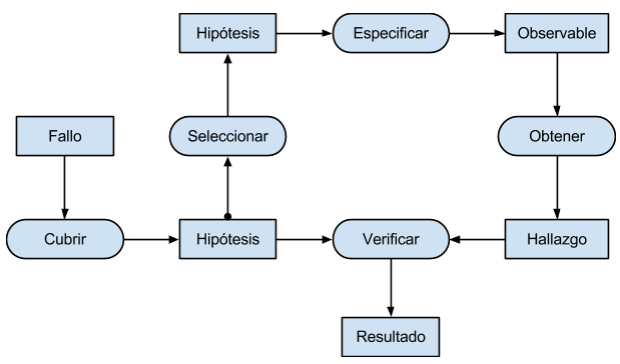
\includegraphics[width=300px]{diagnostico.png} \\
			\subsubsection{Definiciones}
			Las capas que conforman toda obra de arte son las siguientes:
			\begin{itemize}
			  \item \textbf{Soporte:} ensamblaje de madera unidos por clavos, grapas, y
			  espigas a un armazón.
			  \item \textbf{Preparación:} estuco (carga de yeso mate más aglutinante o
			  cola de conejo, puede tener un pigmento para colorearla)
			  \item \textbf{Pintura:} temple al huevo, hecho con yema de huevo y
			  pigmento.
			  \item \textbf{Barniz:} los temples no se barnizan.
			\end{itemize}
			\newpage
			Las causas de los fallos pueden ser extrínsecas o intrínsecas:
			\begin{itemize}
			  \item \textbf{Causas intrínsecas:} las causadas directamente por el
			  material, el cual va envejeciendo poco a poco el solo.
			  \item \textbf{Causas extrínsecas:}
			  \begin{itemize}
			  \item \textbf{Bióticas:} bichos, insectos, bacterias, pequeños mamíferos,
hongos...
 			  \item \textbf{Ambientales:} humedad más temperatura, catástrofes
naturales, fuego, polvo...
 			  \item \textbf{Químicas:} reacciones químicas.
			  \item \textbf{Antrópicas:} el hombre y el uso de la obra.
			  \end{itemize}
			\end{itemize}
			Otras definiciones:
			\begin{itemize}
			\item \textbf{Craquelado:} el craquelado es un fenómeno de deterioro común en
			pinturas antiguas. Consiste en la aparición de grietas, que en los casos más graves llegan a fragmentar la capa de pintura y desembocar en su desprendimiento. Este signo de envejecimiento se suele imitar en muebles y pinturas para darles apariencia antigua.
			\end{itemize}
			\subsubsection{Fallos}
			\begin{center}
				\begin{tabular}{| p{2cm} | p{6cm} | p{3cm} |}
					\hline
					\cellcolor[RGB]{224,233,250}\textbf{Fallo} &
					\cellcolor[RGB]{224,233,250}\textbf{Descripción} &
					\cellcolor[RGB]{224,233,250}\textbf{Hipótesis relacionadas}\\
					\hline
					F01 & El cuadro tiene un tono anormal. & H01, H12, H13, H20, H21, H22,
					H24\\
					\hline
					F02 & La pintura destiñe. & H02, H03\\
					\hline
					F03 & La pintura está craquelada. &
					H04, H05, H06, H07, H09\\
					\hline
					F04 & La pintura está caída. &
					H02, H03, H04, H05, H06, H07, H08, H24\\
					\hline
					F05 & La pintura se disgrega. & H06\\
					\hline
					F06 & Hay elementos indeseables en la pintura. &
					H09, H11, H23\\
					\hline
					F07 & La pintura está curvada o alabeada. & H10\\
					\hline
					F08 & El color del soporte ha cambiado. &
					H12, H13, H14, H15, H16, H18\\
					\hline
					F09 & El estado del soporte ha cambiado. & H15, H17, H19\\
					\hline
				\end{tabular}
			\end{center}
			\newpage
			\subsubsection{Hipótesis}
			\begin{center}
				\begin{tabular}{| p{2cm} | p{6cm} | p{3cm} |}
					\hline
					\cellcolor[RGB]{224,233,250}\textbf{Hipótesis} &
					\cellcolor[RGB]{224,233,250}\textbf{Descripción} &
					\cellcolor[RGB]{224,233,250}\textbf{Observables relacionados}\\
					\hline
\cellcolor[RGB]{224,233,250} & \cellcolor[RGB]{224,233,250}Causa intrínseca - Capa de barniz &
\cellcolor[RGB]{224,233,250}\\
 \hline
H01 & Se ha barnizado el temple. & O01\\
\cellcolor[RGB]{224,233,250} & \cellcolor[RGB]{224,233,250}Causa intrínseca - Capa pictórica &
\cellcolor[RGB]{224,233,250}\\
 \hline
H02 & No se han mezclado los colores bien con el agua al usar un colorante. &
O02\\
\hline
H03 & Hay poco aglutinante en la mezcla. & O02\\
 \hline
H04 & Hay un exceso de aglutinante. & O03\\
 \hline
H05 & La pintura está empastada. & O04\\
 \hline
\cellcolor[RGB]{224,233,250} & \cellcolor[RGB]{224,233,250}Causa intrínseca - Capa de preparación &
\cellcolor[RGB]{224,233,250}\\
 \hline
H06 & Falta aglutinante en la capa de preparación. & O05\\
 \hline
H07 & Sobra aglutinante en la capa de preparación. & O05\\
\cellcolor[RGB]{224,233,250} & \cellcolor[RGB]{224,233,250}Causa intrínseca - Capa de soporte &
\cellcolor[RGB]{224,233,250}\\
 \hline
H08 & Se han usado los nudos y la médula del árbol como soporte que acaban
pudriéndose. & O06\\
 \hline
H09 & Oxidación de elementos metálicos del soporte como grapas... & O07\\
 \hline
H10 & Se han usado refuerzos para impedir el movimiento como colas de milano,
espigas... & O08\\
 \hline
\cellcolor[RGB]{224,233,250} & \cellcolor[RGB]{224,233,250}Causa extrínsecas bióticas - Capa de barniz -
No hay & \cellcolor[RGB]{224,233,250}\\
 \hline
\cellcolor[RGB]{224,233,250} & \cellcolor[RGB]{224,233,250}Causa extrínsecas bióticas - Capa pictórica
&\cellcolor[RGB]{224,233,250}
\\
 \hline
H11 & Los hongos han atacado la pintura. & O09 y O10\\
 \hline
H12 & Algún mamífero ha defecado en la pintura, analizar el excremento en un
laboratorio para identificarlo. & O11\\
 \hline
H13 & Algún ave ha defecado en la pintura, analizar el excremento en un laboratorio
para identificarlo. & O11\\
\hline
\end{tabular}
			\end{center}
			\newpage
			\begin{center}
				\begin{tabular}{| p{2cm} | p{6cm} | p{3cm} |}
					\hline
					\cellcolor[RGB]{224,233,250}\textbf{Hipótesis} &
					\cellcolor[RGB]{224,233,250}\textbf{Descripción} &
					\cellcolor[RGB]{224,233,250}\textbf{Observables relacionados}\\
 \hline
 \cellcolor[RGB]{224,233,250}& \cellcolor[RGB]{224,233,250}Causa extrínsecas bióticas - Capa de
 preparación - No hay & \cellcolor[RGB]{224,233,250}\\
 \hline
 \cellcolor[RGB]{224,233,250}& \cellcolor[RGB]{224,233,250}Causa extrínsecas bióticas - Capa de soporte
 &\cellcolor[RGB]{224,233,250}
 \\
 \hline
H14 & Los hongos han atacado el soporte. & O12\\
 \hline
H15 & Los hongos xilófagos han atacado el soporte. & O12 y O13\\
 \hline
H16 & El soporte ha sido afectado por pudrición parda. & O14\\
 \hline
H17 & El soporte ha sido afectado por pudrición blanda. & O15\\
 \hline
H18 & El soporte ha sido afectado por pudrición blanca. & O14\\
 \hline
H19 & El soporte ha sido atacado por insectos. & O16\\
 \hline
 \cellcolor[RGB]{224,233,250}& \cellcolor[RGB]{224,233,250}Causa extrínsecas ambientales - Capa de barniz
 & \cellcolor[RGB]{224,233,250}\\
 \hline
H20 & El barniz se ha oxidado. & O01\\
 \hline
H21 & Se ha depositado polvo encima del barniz. & O01 y O17\\
 \hline
H22 & El humo de la vela ha ennegrecido el barniz. & O01\\
 \hline
\cellcolor[RGB]{224,233,250} & \cellcolor[RGB]{224,233,250}Causa extrínsecas ambientales - Capa pictórica
& \cellcolor[RGB]{224,233,250}\\
 \hline
H23 & La pintura se ha sometido a calor continuado. & O18\\
 \hline
H24 & Se ha quemado el cuadro. & O01 y O19\\
 \hline
				\end{tabular}
			\end{center}
			\newpage
			\subsubsection{Observables o Preguntas}
			\begin{center}
				\begin{tabular}{| p{2cm} | p{6cm} | p{3cm} |}
					\hline
					\cellcolor[RGB]{224,233,250}\textbf{Observable} &
					\cellcolor[RGB]{224,233,250}\textbf{Descripción} &
					\cellcolor[RGB]{224,233,250}\textbf{Valores relacionados}\\
					\hline
O01 & Comprobar tono del cuadro. & V01, V02 y V03 y V04\\
					\hline
O02 & Pasa la mano por el cuadro. & V05, V06, V07 y V08\\
					\hline
O03 & ¿Observas surcos grasos en la zona craquelada? & V17\\
					\hline
O04 & Comprobar el cuadro de perfil. & V09 y V10\\
					\hline
O05 & Lijar un resto de la capa de preparación a la que le falte pintura. &
V11 y V12\\
					\hline
O06 & ¿Ves un hueco grande y ovalado? & V17\\
					\hline
O07 & ¿Hay algún objeto metálico oxidado debajo de la zona abultada o
craquelada? & V17\\
					\hline
O08 & ¿El cuadro presenta refuerzos, colas de milano o espigas en la parte
trasera? & V17\\
					\hline
O09 & ¿Hay manchas de color gris o azulado en la pintura? & V17\\
					\hline
O10 & ¿Hay pelusilla en la pintura? (Depende de que O09 sea V17) & V17\\
					\hline
O11 & ¿Presenta manchas secas o bolitas pequeñas oscuras? & V13 y V14\\
					\hline
O12 & ¿Hay manchas de color gris o azulado en el soporte? & V17\\
					\hline
O13 & ¿Pesa menos el cuadro? & V17\\
					\hline
O14 & ¿De qué color es el soporte? & V15 y V16\\
					\hline
O15 & ¿El soporte está gelatinoso? & V17\\
					\hline
O16 & ¿Tiene el soporte agujeros limpios de forma circular o elíptica? & V17\\
					\hline
O17 & ¿Manchas de polvo una bayeta al pasarla por el cuadro? (Depende de que O01
sea V03) & V17\\
					\hline
O18 & ¿La pintura tiene ampollas o burbujas? & V17\\
					\hline
O19 & ¿El cuadro tiene zonas donde se ha caído la pintura o está carbonizada?
(Depende de que O01 sea V04) & V17\\
					\hline
				\end{tabular}
			\end{center}
			\newpage
			\subsubsection{Valores, Hallazgos o Respuestas}
			\begin{center}
				\begin{tabular}{| p{2cm} | p{6cm} | p{3cm} |}
					\hline
					\cellcolor[RGB]{224,233,250}\textbf{Valor} &
					\cellcolor[RGB]{224,233,250}\textbf{Descripción} &
					\cellcolor[RGB]{224,233,250}\textbf{Hipótesis que cumple}\\
					\hline
V01 & Tono amarillento. & H01\\
					\hline
V02 & Tono translúcido. & H01\\
					\hline
V03 & Tono opaco. & H20 y H21\\
					\hline
V04 & Tono negro. & H22 y H24\\
					\hline
V05 & Mano manchada de rojo cadmio medio. & H02\\
					\hline
V06 & Mano manchada de amarillo cadmio. & H02\\
					\hline
V07 & Mano manchada de azul esmalte. & H02\\
					\hline
V08 & Mano manchada con varios colores. & H03\\
					\hline
V09 & Zona con grueso de pintura craquelada. & H05\\
					\hline
V10 & Zona con grueso de pintura craquelada y con laguna faltante. & H05\\
					\hline
V11 & Se lija fácilmente. & H06\\
					\hline
V12 & Se lija con dificultad. & H07\\
					\hline
V13 & Bolitas oscuras. & H12\\
					\hline
V14 & Manchas secas. & H13\\
					\hline
V15 & Marrón oscuro. & H16\\
					\hline
V16 & Blanquecino. & H18\\
					\hline
V17 & Si & H04, H08, H09, H10, H11, H14, H15, H17, H19, H21, H23, H24\\
					\hline
				\end{tabular}
			\end{center}
		\newpage
		\subsection{Modelo de comunicación}
			Puesto que para la aplicación desarrollamos una única tarea intensiva en
			conocimiento, esto es el Diagnóstico sobre el estado de las obras de arte,
			hemos considerado que no es necesario llevar a cabo el modelo de
			comunicación.\\
			
			Esta tarea sí conlleva un intercambio de información en su interior pero es
			muy sencillo:
			\begin{enumerate}
				\item La aplicación hace preguntas al usuario. Las preguntas se componen de
				una cadena y se muestran por pantalla.
				\item El usuario responde a la aplicación. La respuesta es una selección en
				un menú desplegable.
				\item La aplicación devuelve sus conclusiones. Estas conclusiones forman una
				lista de cadenas que se muestran por pantalla.
			\end{enumerate}
			Aquí hay un diagrama basado en la tarea de Diagnóstico que ilustraría el
			intercambio de información entre la aplicación y el usuario. No indica el
			orden de las comunicaciones, aunque se puede intuir:\\\\
			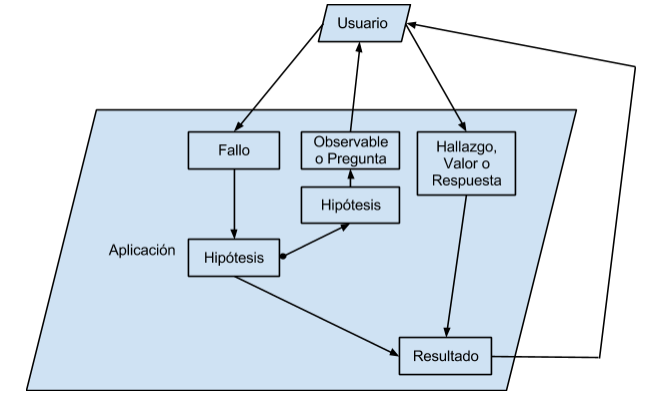
\includegraphics[width=300px]{proceso.png} \\
	\newpage
	\section{Modelado de diseño}
		\subsection{Modelo de diseño}
			\subsubsection{Formulario DM-1}
			\begin{center}
				\begin{tabular}{| l | p{5cm} |}
					\hline
					\cellcolor[RGB]{224,233,250}\textbf{Decisiones arquitectónicas} &
					\cellcolor[RGB]{224,233,250}\textbf{Formato} \\
					\hline
					\cellcolor[RGB]{224,233,250}\textbf{Organización de los subsistemas} & La
					aplicación sigue una arquitectura MVC en un servidor. El Modelo se guarda en un archivo Javascript, el Controlador está programado en Javascript y la Vista en HTML5, CSS3 y Javascript.
					\\
					\hline
					\cellcolor[RGB]{224,233,250}\textbf{Modelo de control} & El modelo de
					control se basa en eventos y en un motor de inferencia simple con encaminamiento hacia adelante basado en hechos y respuestas a preguntas.\\
					\hline
					\cellcolor[RGB]{224,233,250}\textbf{Descomposición de subsistemas} & Se ha
					seguido un paradigma de Orientación a Objetos. No nos hemos visto en la necesidad de hacer diagramas puesto que la aplicación es muy sencilla y parte de ella se ha podido adquirir de terceros.\\
					\hline
				\end{tabular}
			\end{center}
			\newpage
			\subsubsection{Formulario DM-2}
			\begin{center}
				\begin{tabular}{| p{4.8cm} | p{6.5cm} |}
					\hline
					\cellcolor[RGB]{224,233,250}\textbf{Producto software} & SDJS - RCPTTE \\
					\hline
					\cellcolor[RGB]{224,233,250}\textbf{Hardware potencial} & El sistema se va
					a instalar en un servidor web. Es una aplicación sencilla donde el cálculo se realiza en el cliente por lo que el servidor se limita a servir peticiones.\\
					\hline
					\cellcolor[RGB]{224,233,250}\textbf{Hardware de desarrollo} & Para el
					desarrollo del sistema contamos con equipos normales y portátiles de una potencia y costes moderados.\\
					\hline
					\cellcolor[RGB]{224,233,250}\textbf{Librería de visualización} & Para la
					visualización de la aplicación se va a emplear una aplicación web realizada con HTML5, CSS3 y Javascript.\\
					\hline
					\cellcolor[RGB]{224,233,250}\textbf{Lenguaje de implementación} & El
					lenguaje empleado para el motor de inferencia es Javascript. Hemos encontrado un motor de inferencia realizado por Jose Manuel Ayala Wilson y licenciado bajo GNU GPL V3 que podemos reutilizar.\\
					\hline
					\cellcolor[RGB]{224,233,250}\textbf{Representación del conocimiento} & La
					representación del conocimiento se realizará en una base del conocimiento hecha en Javascript y formada por preguntas, respuestas, hechos y reglas.\\
					\hline
					\cellcolor[RGB]{224,233,250}\textbf{Protocolos de interacción} & La
					aplicación sólo es accesible mediante el navegador al ser una página web. Sin embargo tiene un formato que permite su acceso desde PC, Tablet o Smartphone.\\
					\hline
					\cellcolor[RGB]{224,233,250}\textbf{Control de flujo} & El flujo de la
					aplicación consistirá en el uso de un motor de inferencias y una serie de preguntas cuya respuesta almacenará hechos en una base del conocimiento. Eventualmente la aplicación alcanzará una conclusión.\\
					\hline
					\cellcolor[RGB]{224,233,250}\textbf{Soporte para CommonKADS} & Vamos a
					emplear Aptana Studio para el desarrollo de la aplicación web, Git para realizar el proyecto de forma colaborativa y el plugin TeXlipse para Aptana para el desarrollo de los modelos CommonKADS en Latex.\\
					\hline
				\end{tabular}
			\end{center}
			\subsubsection{Formularios DM-3 y DM-4}
			Hemos considerado que no es necesario comentar acerca del motor de
			inferencia, métodos, variables, decisiones de diseño, etc... porque hemos
			reutilizado para nuestra aplicación el motor de inferencia REE en Javascript
			de Jose Manuel Ayala Wilson. Hemos considerado que sería más instructivo
			descargar su aplicación de prueba y acceder a su documentación. Este motor de
			inferencia puede descargarse desde:
			\begin{itemize}
			  \item Su blog en
			  \href{http://jmaw.blogspot.com.es/}{http://jmaw.blogspot.com.es/}
			  \item Página del proyecto en Google Code 
			  \href{https://code.google.com/p/js-ree/}{https://code.google.com/p/js-ree/}
			\end{itemize}
		\section{Conclusión}
		Y con esto acaba la especificación del SDJS - RCPTTE. Si hay algún detalle
		que se nos haya olvidado indicar consulte la documentación de la aplicación o
		asista a la presentación de la misma. Puede acceder a la aplicación en la
		siguiente dirección:
		\begin{itemize}
			  \item
			  \href{http://www.uco.es/~i02arlur/app/}{http://www.uco.es/~i02arlur/app/}
		\end{itemize}
		Puede descargar este documento, la aplicación y la presentación si accede al
		proyecto en GitHub:
		\begin{itemize}
			  \item
			  \href{https://github.com/Elolawyn/ISSBCDiagnostico}{https://github.com/Elolawyn/ISSBCDiagnostico}
		\end{itemize}
\end{document}